\documentclass{report}
\usepackage[utf8]{inputenc} 
\usepackage[russian]{babel} 
\usepackage{enumerate}
\usepackage{fullpage}
\usepackage{indentfirst} 
\usepackage{amsfonts}
\renewcommand{\baselinestretch}{2}
\usepackage{pst-plot}
\usepackage{wrapfig}
\usepackage{xfrac}
\usepackage{listings}
\usepackage{color}
\usepackage{xcolor}
\usepackage{cmap}
\usepackage{spverbatim}
\usepackage{cmap}
\usepackage{tabu}
\usepackage{longtable}
\usepackage{caption}
\usepackage{multicol}
\usepackage{array}
\usepackage{multirow}
\usepackage{fancyvrb}
\usepackage{graphicx}

\usepackage[left=2cm,right=2cm,
    top=2cm,bottom=2cm,bindingoffset=0cm]{geometry}


\definecolor{string}{HTML}{B40000} % цвет строк в коде
\definecolor{comment}{HTML}{008000} % цвет комментариев в коде
\definecolor{keyword}{HTML}{1A00FF} % цвет ключевых слов в коде
\definecolor{morecomment}{HTML}{8000FF} % цвет include и других элементов в коде
%\definecolor{сaptiontextm}{HTML}{FFFFFF} % цвет текста заголовка в коде
%\definecolor{сaptionbk}{HTML}{999999} % цвет фона заголовка в коде
\definecolor{bk}{HTML}{FFFFFF} % цвет фона в коде
\definecolor{frame}{HTML}{999999} % цвет рамки в коде
\definecolor{brackets}{HTML}{B40000} % цвет скобок в коде


 % Настройки отображения кода
\lstset{
language=C++, % Язык кода по умолчанию
 % Цвета
keywordstyle=\color{keyword}\ttfamily\bfseries,
stringstyle=\color{string}\ttfamily,
commentstyle=\color{comment}\ttfamily\itshape,
morecomment=[l][\color{morecomment}]{\#},
 % Настройки отображения.....
breaklines=true, % Перенос длинных строк
basicstyle=\ttfamily\footnotesize, % Шрифт для отображения кода
backgroundcolor=\color{bk}, % Цвет фона кода
frame=lrb,xleftmargin=\fboxsep,xrightmargin=-\fboxsep, % Рамка, подогнанная к заголовку
rulecolor=\color{frame}, % Цвет рамки
tabsize=3, % Размер табуляции в пробелах
 % Настройка отображения номеров строк. Если не нужно, то удалите весь блок
numbers=left, % Слева отображаются номера строк
stepnumber=1, % Каждую строку нумеровать
numbersep=5pt, % Отступ от кода.
numberstyle=\small\color{black}, % Стиль написания номеров строк
}

\usepackage{caption}
\DeclareCaptionFont{white}{\color{white}}
\DeclareCaptionFormat{listing}{\parbox{\linewidth}{\colorbox{gray}{\parbox{\linewidth}{#3}}\vskip-4pt}}
\captionsetup[lstlisting]{format=listing,labelfont=white,textfont=white}


\author{{\huge Мингалёв Олег}\\
Московский государственный университет им. М. В. Ломоносова,\\
Факультет вычислительной математики и кибернетики,\\
101 группа\\
\texttt{oleg@mingalev.net}}
\title{Динамические структуры данных}
\date{10 марта 2014 г.}

\begin{document}
\maketitle
%\addcontentsline{toc}{chapter}{Annexes}
\tableofcontents
\chapter{Постановка задачи}
\section{Формулировка задачи}

Заданы два многочлена, найдите их сумму.

\section{Формат входных данных}

Многочленом считается алгебраическая сумма одночленов вида \texttt{aX\^{}n}, \texttt{aX}, \texttt{X\^{}n} и \texttt{a}, завершённая переводом строки, причём $ a > 0 $, $ n > 1 $. Нулевой многочлен задаётся строкой \texttt{0\textbackslash{}n}.

Формально, \texttt{<poly> ::= ([-]([<num>]X[\^{}<num>]|<num>)((+|-)([<num>]X[\^{}<num>]|<num>)*)|(0))\textbackslash{}n}.

Одночлены одной степени не повторяются.

\section{Формат выходных данных}

Необходимо вывести сумму двух введённых многочленов в формате, описанном в разделе <<Формат входных данных>> по убыванию степеней одночленов.


\chapter{Лексемный анализ}

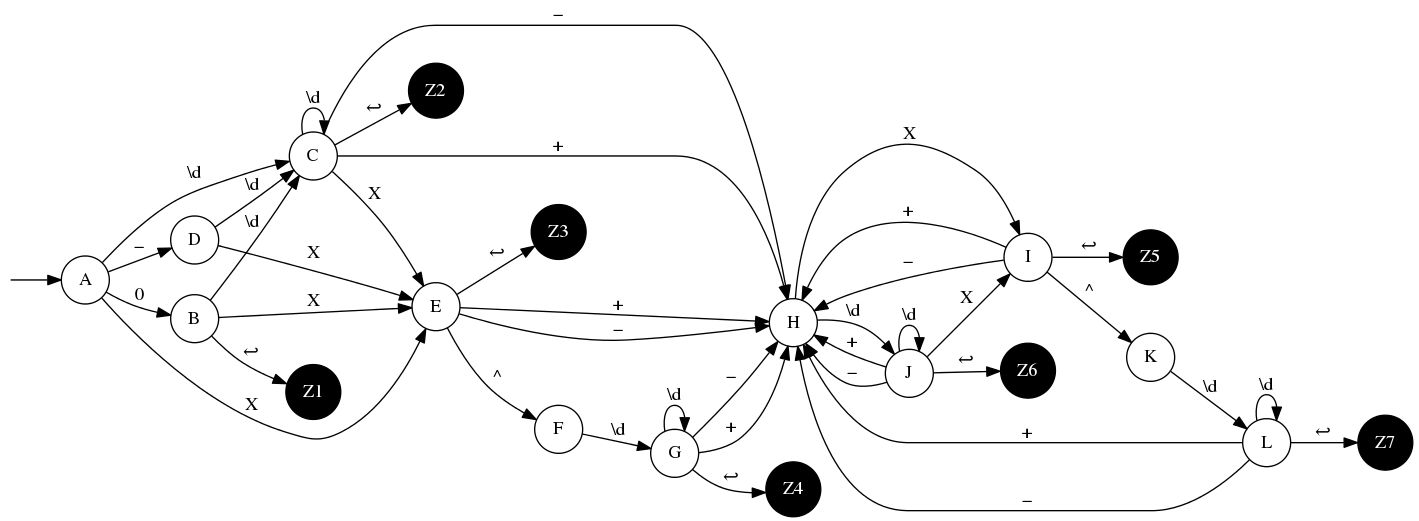
\includegraphics[width=\linewidth]{graph.png}

Синтаксический разбор многочленов представляет из себя моделирование вышепредставленного автомата. Выдененные вершины "--- терминальные.

\chapter{Тестирование}
\begin{Verbatim}[frame=single,baselinestretch=0.5]
[shhdup@shhdup-think lab02]$ ./lab02 
lab02 v0.0.4, Mingalev Oleg 2014

Use lab02 -h to see help page

Variant: 16
Sum of two polynomials
================================
1st poly: X^2+X+1
2nd poly: X^2+X-1
Sum: 2X^2+2X
[shhdup@shhdup-think lab02]$ ./lab02 
lab02 v0.0.4, Mingalev Oleg 2014

Use lab02 -h to see help page

Variant: 16
Sum of two polynomials
================================
1st poly: X^2+2X
2nd poly: -X^2-3X+10
Sum: -X+10
[shhdup@shhdup-think lab02]$ ./lab02 
lab02 v0.0.4, Mingalev Oleg 2014

Use lab02 -h to see help page

Variant: 16
Sum of two polynomials
================================
1st poly: X^12+16X 
2nd poly: 0
Sum: X^12+16X
[shhdup@shhdup-think lab02]$ ./lab02 
lab02 v0.0.4, Mingalev Oleg 2014

Use lab02 -h to see help page

Variant: 16
Sum of two polynomials
================================
1st poly: 0
2nd poly: 0
Sum: 0
[shhdup@shhdup-think lab02]$ ./lab02 
lab02 v0.0.4, Mingalev Oleg 2014

Use lab02 -h to see help page

Variant: 16
Sum of two polynomials
================================
1st poly: -X^3+X^2+1
2nd poly: -1-X^2+X^3
Sum: 0
\end{Verbatim}

\newpage

\begin{Verbatim}[frame=single,baselinestretch=0.5]
[shhdup@shhdup-think lab02]$ ./lab02 
lab02 v0.0.4, Mingalev Oleg 2014

Use lab02 -h to see help page

Variant: 16
Sum of two polynomials
================================
1st poly: +X^2+X
Syntax error at position 1: Symbols {-0123456789X} excepted but '+'[43] found
[shhdup@shhdup-think lab02]$ ./lab02 
lab02 v0.0.4, Mingalev Oleg 2014

Use lab02 -h to see help page

Variant: 16
Sum of two polynomials
================================
1st poly: X^2+X^1
Error: Powers should be at least 2
[shhdup@shhdup-think lab02]$ ./lab02 
lab02 v0.0.4, Mingalev Oleg 2014

Use lab02 -h to see help page

Variant: 16
Sum of two polynomials
================================
1st poly: 2X^3+3X+23X^3
Error: At least two monominals with power 3
[shhdup@shhdup-think lab02]$ ./lab02 
lab02 v0.0.4, Mingalev Oleg 2014

Use lab02 -h to see help page

Variant: 16
Sum of two polynomials
================================
1st poly: 0X+2
Error: Multipliers must be nonzero
[shhdup@shhdup-think lab02]$ ./lab02 
lab02 v0.0.4, Mingalev Oleg 2014

Use lab02 -h to see help page

Variant: 16
Sum of two polynomials
================================
1st poly: X^X
Syntax error at position 3: Symbols {0123456789} excepted but 'X'[88] found
[shhdup@shhdup-think lab02]$ ./lab02 
lab02 v0.0.4, Mingalev Oleg 2014

Use lab02 -h to see help page

Variant: 16
Sum of two polynomials
================================
1st poly: 12*X
Syntax error at position 3: Symbols {\n0123456789X+-} excepted but '*'[42] found
[shhdup@shhdup-think lab02]$ ./lab02 
lab02 v0.0.4, Mingalev Oleg 2014

Use lab02 -h to see help page

Variant: 16
Sum of two polynomials
================================
1st poly: XX^2
Syntax error at position 2: Symbols {\n^+-} excepted but 'X'[88] found
[shhdup@shhdup-think lab02]$ ./lab02 
lab02 v0.0.4, Mingalev Oleg 2014

Use lab02 -h to see help page

Variant: 16
Sum of two polynomials
================================
1st poly: X^2+
Syntax error at position 5: Symbols {X0123456789} excepted but new line found

\end{Verbatim}


\appendix
\chapter{Исходный код}

\lstinputlisting[caption=Makefile]{../lab02.c}

\end{document}
